
\chapter{系统配置}
\label{chap:systemConfig}

\rule[0pt]{\textwidth}{0.1pt}

在对系统进行进一步的配置之前,先学习关于系统的组织结构以及文件或程序的
查找方法不失为一个不错的选择。我们还会介绍如何自己编译内核,如果你正打
算这么做的话,本章应该很有帮助。本章的主要内容是让你了解系统的组织结构
及相关的配置文件。之后我们就可以配置系统的更为高深的部分了。

\section{系统一览}
\label{sec:systemConfig:systemOverview}

在对Linux分解认识之前,了解Linux系统的组成方式无疑是极其重要的。Linux
系统与DOS、Windows或是Macintosh(类Unix的Mac OS X例外)等系统有着显著
的不同,我们会在下面的几节中帮助你了解Linux的布局,从而使你能够根据自
己的需求来配置系统。

\subsection{文件系统布局}
\label{sec:systemConfig:systemOverview:fileSystemLayout}

Slackware Linux与DOS或者Windows的第一个显著差别就是文件系统。首先,我
们并不使用驱动器的盘符来表示分区。在Linux下,有一个主目录,我们可以类
比为DOS下的\texttt{C:}盘。并且系统中的每个分区都挂载到该主目录的某个子
目录下。听起来有点像是一个可以无限扩展的硬盘。

我们将这个主目录称为\texttt{root}目录,并用一个斜杆(/)来表示。这个概
念开始时可能不好理解,甚至有些诡异,但当我们需要增加更多的空间时,这个
设计的优势就能很好地体现出来了。例如,我们假设有个硬盘,挂载到
\texttt{/home}目录的某个子目录上,它的空间已经用完了。虽然大多数人在安
装Slackware时都分配了一个较大的root分区。由于分区可以被挂载到任意目录
下,所以我们可以随意到商店中买一块新的硬盘,并挂载到\texttt{/home}目录
下,万事OK!现在,我们的系统中就添加了新的空间,整个过程异常简单。

下面,我们要对``\texttt{/}''目录下的主要顶级目录夹进行一个简要的介绍。
\begin{description}
\item[bin] \hfill \\
  该目录下存放一些必需的程序。它包含使用系统的最低要求下的一些程序。该
  文件夹下包括了如shell及一些文件系统的命令(\texttt{ls}、\texttt{cp}
  等等)。在安装之后,一般就不再对\texttt{/bin}目录进行改动。即使进行
  改动,一般也是由官方的更新所做出的改动。
\item[boot] \hfill \\
  该目录存在LILO所需的一些文件。Slackware的内核文件也存放于此。该目录
  在安装后可能会做一些小的改动。
\item[dev] \hfill \\
  在Linux中,一切皆文件,诸如串口、硬盘或扫描仪等设备文件也以文件的形
  式表示。所有的设备节点都存放于\texttt{/dev}目录下。在许多类Unix的系
  统中都采用了这种策略。
\item[etc] \hfill \\
  该目录下存放系统的配置文件。从X的配置文件、用户数据库,到系统的启动
  脚本,都存放于此。随着使用Slackware时间的增长,系统管理员会对该目录越
  来越熟悉。
\item[home] \hfill \\
  Linux是一个多用户系统,每个用户都有一个帐户和一个独立的文件夹来存放
  私人文件,这个文件夹就被称为用户的主目录,默认情况下,它就存放于
  \texttt{/home}目录下。
\item[lib] \hfill \\
  该目录用于存放一些基本操作所依赖的库文件。包括C库、动态链接库、
  ncurse库及内核模块等等。
\item[media] \hfill \\
  一些设备的默认挂载点。包括CDROM、DVD等的挂载点。
\item[mnt] \hfill \\
  该目录的作用是作为硬盘或可移动设备的临时挂载目录。其中包括CDROM及软
  盘的挂载点。注意,该目录与\texttt{/media}的区别在于该目录一般用于临
  时挂载,而\texttt{/media}一般作为默认挂载点。
\item[opt] \hfill \\
  该目录用于安装额外的一些软件包。其中的思想是:将软件包安装到
  \texttt{/opt/software-package}目录下,之后只需要将该目录删除即可卸载
  该软件包。一般而言,将一些占用空间较大的软件包安装到这里(如
  google-chrome、matlab、libreoffice及texlive等)。
\item[proc] \hfill \\
  该目录是个特殊的目录。严格来说,它不属于文件系统的一部分,它是一个虚
  拟的文件系统,为我们提供内核的相关信息。内核需要让我们知道的信息会保
  存为文件的形式,并存放在\texttt{/proc}文件夹内。我们也可以通过修改这
  些文件来向内核传递信息。例如我们可以执行\texttt{cat /proc/cupinfo}来
  获取CPU相关的信息。
\item[root] \hfill \\
  还记得系统管理员的用户名是什么吗?是的,\texttt{root}。与普通用户不
  同的是,\texttt{root}用户的主目录并不存放在\texttt{/home/root}中,而
  是放在\texttt{/root}下。这么做的原因很简单,试想,如果\texttt{/home}
  与\texttt{/}在不同的分区下,那么当\texttt{/home}不能挂载时会发生什么
  情况?很自然地,我们会以\texttt{root}用户登陆并对系统进行修复,那么
  如果它的主目录就在损坏的文件系统上,那么甚至连登陆都成了问题。
\item[sbin] \hfill \\
  在启动过程中,\texttt{root}用户需要用到的一些程序就存放在这个文件夹
  中。普通用户不会用到该目录下的程序。
\item[tmp] \hfill \\
  该目录为临时存储的文件夹。所有用户都有对该目录的读写权限。
\item[usr] \hfill \\
  该目录在Linux系统中是个相当大的目录。除了上面提到的东西外,其它的内
  容一般都放在该文件夹下,包括程序、文档、内核源码及X Window系统等。一
  般情况下,我们会将软件安装到该文件夹下。
\item[var] \hfill \\
  该目录用于存放系统日志、缓冲的数据及程序锁文件等。该目录的内容最常改
  变。
\end{description}
现在你应该有些印象了,系统有什么文件夹,什么样的文件夹中放什么东西。如
果你想更详细了解文件系统的布局,可以参见\texttt{hier\textbf{(7)}}的man
手册。下一节中,我们会讲解如何快速地查找文件,之后就不需要人工地查找了。

\subsection{查找文件}
\label{sec:systemConfig:systemOverview:findingFiles}
现在我们知道了系统一些主要文件夹的功能,但这并不能真正帮我们找到一些特
定的文件。是的,我们可以一个个文件夹地查找,但我们需要的是快速地查找。
Slackware中有四个主要的文件搜索命令。

\subsubsection{which}
\label{sec:systemConfig:systemOverview:findingFiles:which}

我们首先要介绍的就是\texttt{which\textbf{(1)}}命令。\texttt{which}一般
用于快速定位某个程序的位置。它的作用是查找我们的环境变量\texttt{PATH},
并返回第一个搜索到的路径。例如:
\begin{Verbatim}[frame=single, commandchars=\\\{\}]
  \% \textbf{which bash}
  /bin/bash
\end{Verbatim}
从上例中我们可以看到,\texttt{bash}位于\texttt{/bin}目录中。对于搜索而
言,\texttt{which}的功能有限,因为它只对\texttt{PATH}进行搜索。


\subsubsection{whereis}
\label{sec:systemConfig:systemOverview:findingFiles:whereis}

接下来介绍命令\texttt{whereis\textbf{(1)}}。它与\texttt{which}类似,只
是它除了搜索\texttt{PATH}外,还对man手册进行搜索,我们使用
\texttt{whereis}对\texttt{bash}命令进行搜索时,它还返回如下结果:
\begin{Verbatim}[frame=single, commandchars=\\\{\}]
\% \textbf{whereis bash}
bash: /bin/bash /usr/bin/bash /usr/man/man1/bash.1.gz
\end{Verbatim}
\texttt{whereis}命令不仅告诉我们程序的实际位置,还告诉我们相应的文档的
位置。但,一样的,该命令的功能有限。如果我们只想查找一个特定配置文件的
位置呢?显然使用\texttt{which}或\texttt{whereis}命令都无法解决这个问题。


\subsubsection{find}
\label{sec:systemConfig:systemOverview:findingFiles:find}
下面介绍\texttt{find\textbf{(1)}}命令,它是一个功能异常强大的命令。我
们可以指定一定的搜索规则对文件系统进行搜索。例如可以使用文件名通配符、
指定文件的创建或修改时间或都其它的一些规则。举个例子,如果我们想搜索系
统中默认的\texttt{xinitrc}文件的位置,我们可以使用如下命令:
\begin{Verbatim}[frame=single, commandchars=\\\{\}]
\% \textbf{find / -name xinitrc}
/etc/X11/xinit/xinitrc
\end{Verbatim}
由于上述的\texttt{find}命令是对整个文件系统进行遍历搜索,所以要花上相
当长的一段时间。并且,如果使用普通用户执行命令,在搜索那些只有
\texttt{root}用户能看到的文件夹时,还会出现``权限不足''的错误,但最重
要的是它的确找到了我们想要的文件。尽管如此,要是能再快一点就好了……


\subsubsection{slocate}
\label{sec:systemConfig:systemOverview:findingFiles:find}
和\texttt{find}一样,\texttt{slocate\textbf{(1)}}也是对整个文件系统进
行搜索,但它搜索的并不是真正的文件系统,而是一个事先生成的数据库。该数
据库默认在每天凌晨时自动更新。但对于一些个人用户,凌晨时电脑一般处于关
机状态,所以,我们可以手动执行\texttt{updatedb\textbf{(1)}}命令来更新
数据库(执行该命令需要\texttt{root}权限,使用\texttt{su}命令切换到
\texttt{root}用户或使用\texttt{sudo}即可获得\texttt{root}权限)。下面
我们举个例子:
\begin{Verbatim}[frame=single, commandchars=\\\{\}]
\% \textbf{slocate xinitrc} \# 这里并不需要root权限
/etc/X11/xinit/xinitrc
/etc/X11/xinit/xinitrc.fluxbox
/etc/X11/xinit/xinitrc.fvwm2
/etc/X11/xinit/xinitrc.twm
/etc/X11/xinit/xinitrc.xfce
/etc/X11/xinit/xinitrc.kde
...
\end{Verbatim}
得到的结果很长,但是运行速度很快。使用以上这些命令,我们就能够快速地找
到我们想查找的文件了。

\subsection{\texttt{/etc/rc.d}文件夹}
\label{sec:systemConfig:systemOverview:etcRcd}
\texttt{/etc/rc.d}文件夹用于存放系统的初始化文件。与System V采用init脚
本的方法不同,Slacwkare为它的初始化文件采用了BSD风格的布局。init脚本的
风格在不借助专门为此设计的软件时,配置起来是很困难的。对于BSD风格的初
始化脚本,每个运行级别都有一个单独的rc文件,而System V中,每个运行级别
都有自己的一个目录,每个目录下又包含多个init脚本,采用这种设计维护进行
比较方便。

初始化文件可以分为很多类别。有系统启动、运行级别、网络初始化及System V
兼容等。对于每个类别,我们都会将其它东西归为另一个类别。(As per
tradition, we'll lump everything else into another category.)


\subsubsection{系统启动}
\label{sec:systemConfig:systemOverview:etcRcd:systemStartup}

除了内核之外,Slackware运行的第一个程序是\texttt{init\textbf{(8)}}。该
程序读取文件\texttt{/etc/inittab}中的配置告诉自己如何启动系统。在进行
指定的运行级别之前,\texttt{init}执行\texttt{/etc/rc.d/rc.S}脚本,为系
统作好准备。\texttt{rc.S}文件的作用是启用虚拟内存,挂载文件系统,清理
一些特定的日志文件夹,初始化热插拔设备,载入内核模块,配置PCMCIA设备,
设置串口,并执行System V的启动脚本(如果有的话)。很显然,
\texttt{rc.S}做了很多工作,下面是一些\texttt{rc.S}调用的脚本,它们都位
于\texttt{/etc/rc.d}目录下:

\begin{description}
\item[rc.S] \hfill \\
  系统真正的初始化脚本。
\item[rc.modules] \hfill \\
  该脚本用于载入内核模块。如网卡、PPP设备及其它的一些模块。如果该脚本
  找到\texttt{rc.netdevice}文件,\texttt{rc.modules}也会执行它。
\item[rc.pcmcia] \hfill \\
  查找并配置系统中的PCMCIA设备。这对于笔记本用户可能最为有用,因为它们
  的调制解调器或网卡可能就是PCMCIA的\footnote{这里的描述与前面选择启动
    脚本的描述不符,笔者对PCMCIA没什么概念,弄懂了再改吧}。
\item[rc.serial] \hfill \\
  执行适当的\texttt{setserial}命令对串口进行适当的配置。
\item[rc.sysvinit] \hfill \\
  查找与运行级别相关的System V初始化脚本并运行。在下面会进行更详细的介
  绍。
\end{description}

\subsubsection{运行级别初始化脚本}
\label{sec:systemConfig:systemOverview:etcRcd:runlevelInit}

系统初始化结束后,\texttt{init}会继续作运行级别的初使化。所谓的运行级
别是对系统将要运行的状态的描述。听起来很繁琐?好吧,运行级别就是告诉
\texttt{init},是支持多用户还是只支持单用户;要不要开启网络支持;是使
用X Window还是使用\texttt{agetty\textbf{(8)}}来管理登陆。下面的文件定
义了Slacwkare中的不同运行级别。

\begin{description}
\item[rc.0] \hfill \\
  关机(运行级别为0)。默认情况下,该文件是\texttt{rc.6}的一个软链接。
\item[rc.4] \hfill \\
  带有多用户支持启动(运行级别为4),并使用X11的KDM、GDM或XDM作为登陆
  管理器。
\item[rc.6] \hfill \\
  重启系统(运行级别为6)。
\item[rc.K] \hfill \\
  启动单用户模式(运行级别为1)。
\item[rc.M] \hfill \\
  多用户模式(运行级别为2或3),使用传统的基于文本的登陆管理器,这也是
  Slacwkare默认的运行级别。
\end{description}

\subsubsection{网络初始化}
\label{sec:systemConfig:systemOverview:etcRcd:runlevelInit}

运行级别为2、3或4时都会开启网络支持。下面这些文件就是用于网络的初始化
的:

\begin{description}
\item[rc.inet1] \hfill \\
  由\texttt{netconfig}命令生成,该文件用于配置实际使用的网络接口。
\item[rc.inet2] \hfill \\
  在\texttt{rc.inet1}之后执行,并开启基本的网络服务。
\item[rc.atalk] \hfill \\
  启动AppleTalk服务。
\item[rc.http] \hfill \\
  开启Apache网络服务器。与其它脚本相同,只要向它传递stop、start或
  restart参数,就可以相应地停止、启动或重启Apache服务。
\item[rc.news] \hfill \\
  启动新闻服务器。
\end{description}


\subsubsection{System V兼容化}
\label{sec:systemConfig:systemOverview:etcRcd:systemVCompatibilily}

在Slackware 7.0时引入了System V初始化脚本的兼容措施。许多其它的Linux发
行版都采用System V风格的初始化布局而不是BSD风格的。System V为每一个运
行级别的初始化脚本准备了一个文件夹,而BSD风格则是为每个运行级别准备了
一个初始化脚本文件。

脚本\texttt{rc.sysvinit}会搜索存放在\texttt{/etc/rc.d}文件夹下的System
V初始化脚本文件,并执行相应运行级别的脚本。这个兼容性措施对一些安装
System V初始化脚本的商业软件包而言是很重要的。

\subsubsection{其它文件}
\label{sec:systemConfig:systemOverview:etcRcd:otherFiles}
下面介绍的脚本文件是其它的一些初始化脚本。它们一般会通过上面介绍的脚本
的调用运行,所以我们只需要修改这些脚本的内容即可。
\begin{description}
\item[rc.gpm] \hfill \\
  启动文本终端下的鼠标服务。开启后就可以在文本终端下进行复制与粘贴。极
  少数情况下,gpm会引发在X Window下使用鼠标的一些问题。所以如果在使用X
  window时遇到一些鼠标问题,可以尝试去掉该脚本的执行权限并停止gpm服务
  器。
\item[rc.font] \hfill \\
  为文本终端加载自定义字体。(在安装过程中可进行设置。)
\item[rc.local] \hfill \\
  包含你系统独有的一些初始化命令。在安装后该文件是空的,因为它是为系统
  管理员准备的。所有的初始化步骤结束后,系统会执行该脚本。
\end{description}

要启用某个脚本,只需要使用\texttt{chmod}命令为其添加执行权限。相应的,
要停用某个脚本,也只需要去除相应脚本的执行权限即可。关于\texttt{chmod}
命令的更多信息,请参见第//TODO:Section 9.2//节。

\section{选择内核}
\label{sec:systemConfig:selectingAKernel}
内核在一个操作系统中起着至关重要的作用,它提供了对硬件的访问、对进程的
控制以及整个系统的控制。内核中包含了对硬件设备的支持,所以在安装的时候
选择合适的内核是很重要的。

Slackware提供了不止一打的提前编译好的内核可供选择,每个内核都包含一个
标准的驱动集合和一些特定的驱动。你可以选择直接使用提前编译的内核或从源
码编译自己的内核。不管使用哪种方法,都要确保内核中包含系统所需的所有硬
件支持。

\subsection{Slackware CD-ROM上的/kernels文件夹}
\label{sec:systemConfig:selectingAKernel:kernelsDirctory}

提前编译的内核可以在Slackware的CD或DVD上或FTP站点上的Slackware文件夹下
的\texttt{/kernels}文件夹中找到。新的版本发布后,其中可用的内核也会发
生改变,而该文件夹下的文档则是权威的。\texttt{/kernels}文件夹为每个内
核准备了一个子文件夹,每个子文件夹的名字都与它们对应的启动盘名相同。在每
个子文件夹中,你会找到以下文件:
\begin{table}[htpb]
  \centering
  \begin{tabular}{r|l}
    \hline\hline 
    文件名 & 作用 \\ \hline
    System.map & 内核的系统映射文件 \\
    bzImage & 内核本体 \\
    config & 内核源码配置文件  \\
    \hline\hline
  \end{tabular}
  \caption{kernel文件夹中的文件}
  \label{tab:kernelFiles}
\end{table}

要使用一个内核,将\texttt{System.map}及\texttt{config}文件拷贝到
\texttt{/bot}目录中,并将内核镜像\footnote{kernel image,image不知道应
  该怎么翻才好。}复制到\texttt{/boot}文件夹下,重命名为
\texttt{vmlinuz},之后,运行\texttt{/sbin/lilo\textbf{(8)}}命令为
新的内核安装LILO,重启即可。这就是安装一个新内核的步骤。

接下来的内容是过时的。以.i结尾的内核是为IDE设备准备的,这些内核不支持
对SCSI。以.s结尾的内核为SCSI内核,支持IDE,同时支持SCSI。

\subsection{从源码编译内核}
\label{sec:systemConfig:selectingAKernel:compilingAKernel}

新手们常问的一个问题是``我需要自己编译一个内核吗?''。答案是也也许吧。
有一些情况下是需要为自己的系统编译内核的。多数用户只需使用编译好的内核,
外加一些可加载的内核模块就可以构建一个可用的系统了。如果你想使用一个
Slackware当前不提供的新的内核版本,或者你想对内核添加补丁以获取对一些
当前内核不支持的设备的支持,那么你可能需要为自己的系统重新编译内核。如,
一些有SMP功能的系统就会考虑编译一个带SMP支持的内核。许多用户还会自己编
译内核来让机器跑得更快些。要是想针对某些特定的处理器做优化,编译内核也
是有帮助的。

编译自己的内核其实并不难。首先是确保你的机器上安装了内核的源码。即安装
是切记选择安装K系列下的软件包。当然,也要确保安装了D系列的软件包,我们
需要的是D系列中的C编译器、GNU make、及GNU binutils。一般而言,如果做的
工作与开发有关,那么把D系列的软件包全装上会是个不错的选择。你也可以从
\url{http://www.kernel.org/mirrors}网站下载最新的内核源码。


\subsection{2.4.x版本的内核编译}
\label{sec:systemConfig:selectingAKernel:2_4_x}
\begin{Verbatim}[frame=single, commandchars=\\\{\}]
\% \textbf{su -}
Password:
\# \textbf{cd /usr/src/linux}
\end{Verbatim}

第一个步骤是让内核处于默认的状态。使用下面的命令(注意,该命令会删除
\texttt{.config}文件,且没有任何提示,需要的话,可以先进行备份):
\begin{Verbatim}[frame=single, commandchars=\\\{\}]
\# \textbf{make mrproper}
\end{Verbatim}

接下来,我们就可以根据自己的系统来配置内核了。当前的内核提供三种方式。
第一种基于文本的问答系统,它会问用户一系列问题并根据用户的回答来创建配
置文件。这个方法的一个问题就是如果你搞杂了,就得重新来过。多数人选择的
是第二种方式——基于菜单的方式。第三种是基于X的配置工具。选择好你喜欢的
方式,通过执行下面对应的命令即可:
\begin{Verbatim}[frame=single, commandchars=\\\{\}]
  \# \textbf{make config}     (基于文本的问答系统)
  \# \textbf{make menuconfig} (基于文本的菜单驱动系统)
  \# \textbf{make xconfig}    (基于X的版本,请先确保自己在使用X系统)
\end{Verbatim}

\begin{figure}[htpb]
  \centering
  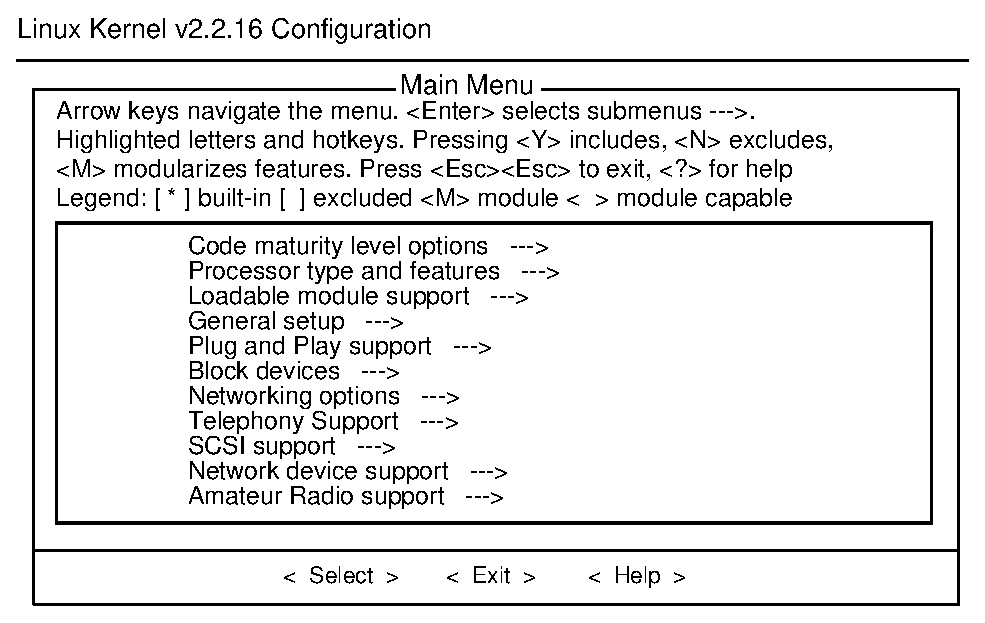
\includegraphics[width=0.8\textwidth]{images/selectingKernel/make-menuconfig.eps}
  \caption{内核配置菜单}
  \label{fig:make-menuconfig}
\end{figure}

对于新用户而言,\texttt{menuconfig}应该是最容易使用的方式。其中提供了
帮助,解释了内核各部分的功能。配置完成后退出配置程序。它会创建一个必要
的配置文件。之后我们就可以准备用来编译的源码树了:
\begin{Verbatim}[frame=single, commandchars=\\\{\}]
  \# \textbf{make dep}
  \# \textbf{make clean}
\end{Verbatim}

下个步骤就是编译内核。首先尝试如下命令:
\begin{Verbatim}[frame=single, commandchars=\\\{\}]
  \# \textbf{make bzImage}
\end{Verbatim}

根据你的CPU速度,这个命令会跑上一会。编译的过程中会显示一些编译器的信
息。编译完成之后,我们还需要编译之前配置时标记为模块的部分。
\begin{Verbatim}[frame=single, commandchars=\\\{\}]
  \# \textbf{make modules}
\end{Verbatim}

接下来就是安装刚编译好的内核了。要在Slackware系统上安装内核,可以使用
如下的命令:
\begin{Verbatim}[frame=single, commandchars=\\\{\}]
  \# \textbf{mv /boot/vmlinuz /boot/vmlinuz.old}
  \# \textbf{cat arch/i386/boot/bzImage > /boot/vmlinuz}
  \# \textbf{mv /boot/System.map /boot/System.map.old}
  \# \textbf{cp System.map /boot/System.map}
  \# \textbf{make modules_install}
\end{Verbatim}
之后是重新配置LILO加载新的内核。首先修改\texttt{/etc/lilo.conf}文件并
为老的内核添加相应的启动项。完成后运行\texttt{/sbin/lilo}来安装新的启
动块。最后重启并以新的内核启动即可。


\subsection{2.6.x版本的内核编译}
\label{sec:systemConfig:selectingAKernel:2_6_x}
2.6版本的内核编译与2.4或2.2的内核只有小部分的区别,但在深究之前了解其
中的差异还是很有必要的。编译2.6内核时,不再需要运行\texttt{make dep}及
\texttt{make clean}了,并且在2.6系列内核中,编译时不再像之前的版本一
亲显示很详细的信息。结果就是编译过程更容易理解了,当然,这样做也有一些
短处。所以如果在编译过程中出了什么错误,我们强烈建议你选择显示详细信息。
只要在编译时加上\texttt{V=1}选项即可。显示更为详细的信息有助于内核开发
人员记录更多信息,在别的geek帮助你时也能更有效率。
\begin{Verbatim}[frame=single, commandchars=\\\{\}]
  \# \textbf{make bzImage V=1}
\end{Verbatim}


\subsection{使用内核模块}
\label{sec:systemConfig:selectingAKernel:usingKernelModules}

内核模块可以认为是设备驱动的一个别名,我们可以在内核运行时对其动态加载
与卸载。通过内核模块,我们在不选择另一个内核或自己编译内核的情况下就能
添加对新硬件的支持。

模块可以在任何时刻进行加载或卸载。这使得系统管理员在更新一些特定驱动时
变得很容易。编译新的模块 --> 卸载旧的模块 --> 加载新的模块,连重启系统
都不需要。

所有的模块都存储在\texttt{/lib/modules/kernel-version}目录下
(kernel-version处根据你的系统而定)。它们可以通过\texttt{rc.modules}
文件在启动时就加载。这个文件的注释很很,并为主要的硬件提供了配置的实例。
使用\texttt{lsmod\textbf{(1)}}可以显示当前活动的模块:
\begin{Verbatim}[frame=single, commandchars=\\\{\}]
  \# \textbf{lsmod}
  Module        Size    Used by
  parport_pc    7220     0
  parport       7844     0   [parport_pc]
\end{Verbatim}
就上面的例子而言,可以看到我只加载了并口的模块。要移除一个模块,使用
\texttt{rmmod\textbf{(1)}}命令。加载模块可以使用
\texttt{modprobe\textbf{(1)}}或\texttt{insmod\textbf{(1)}}命令。其中,
\texttt{modprob}更为安全,因为它解决了模块间的依赖关系。

多数用户从来没有手工加载过模块。他们只使用内核自动加载器(the kernel
autoloader)来管理模块。默认情况下,Slackware的内核中包括了
\texttt{kmod}。\texttt{kmod}是一个内核选项,它使内核在需要时能自动加载
所需的模块。想了解更多关于\texttt{kmod}及如何配置的内核,请参见
\texttt{/usr/src/linux/Documentation/kmod.txt}\footnote{Slackware
  13.37、内核2.6.37中已经找不到该文件。}。再次,前提是你已经安装了内核
源码软件包,或者可以从\url{http://kernel.org}网站上下载内核源码。

我们可以在上面涉及到的命令的相应man手册中找到更多信息,当然,还有
\texttt{rc.modules}文件的相关内容。







%%% Local Variables: 
%%% mode: latex
%%% TeX-master: "../SlackGuide"
%%% End: 
